\section*{Reusability}

\subsection*{Five cancer cohorts and 400 frozen test sets}

We combined breast invasive carcinoma (BRCA), esophageal carcinoma (ESCA), head and neck squamous cell carcinoma (HNSCC), lung squamous cell carcinoma (LSCC) and lung adenocarcinoma (LUAD) from TCGA and CPTAC, 3,238 patients in total (Fig.~\ref{fig:roadmap}b and Table~\ref{tab:cohorts}).\citep{tcga2012brca,tcga2017esca,tcga2015hnsc,tcga2012lusc,tcga2014luad,liu2018clinical,li2023pancancer} The original TCGA marker papers profiled fewer tumours than these cohorts contain (825 breast, 164 oesophageal, 279 head and neck, 178 squamous lung and 230 lung adenocarcinomas),\citep{tcga2012brca,tcga2017esca,tcga2015hnsc,tcga2012lusc,tcga2014luad} so our counts reflect the later PanCancer Atlas and CPTAC data and not those publications. The cohorts are also internally heterogeneous: the oesophageal cohort spans histological subtypes and the head and neck cohort spans HPV-positive and HPV-negative tumours from different anatomical sites.\citep{tcga2017esca,tcga2015hnsc} Patients censored before a horizon cannot be labeled, which left 1,645 patients for 3-year survival, 1,168 for 5-year survival and 937 for an exploratory extreme-survival endpoint that compares death within 3 years with survival beyond 5 years (Fig.~\ref{fig:roadmap}c).

This defines 16 prediction tasks: 13 cancer-specific tasks and three pooled endpoints. Each was split into five repeats of five patient-grouped folds, and the resulting 400 test sets were frozen before any model was run. In the pooled 3-year task, each model was fitted on about 1,050 patients and tested on about 330 per split (Fig.~\ref{fig:roadmap}d). Cancer-specific test sets were much smaller, usually fewer than 70 patients.

\begin{table}[ht]
\centering
\caption{Cancer cohort size and endpoint eligibility. Extreme survival contrasts death within 3 years against survival beyond 5 years. NA, endpoint-specific cohort not formed.}
\label{tab:cohorts}
\begin{tabular}{lrrrr}
\toprule
Cohort & Raw & 3-year eligible & 5-year eligible & Extreme eligible \\
\midrule
BRCA & 1206 & 501 & 350 & 268 \\
ESCA & 182 & 86 & NA & NA \\
HNSCC & 631 & 385 & 286 & 244 \\
LSCC & 595 & 355 & 281 & 222 \\
LUAD & 624 & 318 & 251 & 203 \\
\bottomrule
\end{tabular}

\end{table}

\subsection*{Within a single cancer, no model wins decisively}

Modeled one cancer at a time, survival was hard for every method (Fig.~\ref{fig:within}a). A foundation model had the highest mean ROC AUC in 7 of the 13 tasks, sometimes by a useful margin: in breast cancer extreme survival, TabPFN v2.6 reached 0.613 against 0.569 for the best classical model. Where foundation models trailed, they trailed by at most 0.024. Fold-matched differences from random forest were centered near zero for every nonlinear model (Fig.~\ref{fig:within}b).

Ranked across the 13 tasks, TabPFN v2.5 had the best mean rank (4.8), followed by TabPFN v2 (5.1) and random forest (5.2; Fig.~\ref{fig:within}c). The models differed overall (Friedman $\chi^2 = 20.3$, $P = 0.026$), but the difference came from logistic regression (mean rank 9.4). No two of the ten nonlinear models differed by more than the Nemenyi critical difference of 4.19 ranks.\citep{demsar2006statistical} In this setting TabPFN is reusable: it installs and runs without tuning and performed comparably to default-setting tree ensembles. A non-significant difference is not evidence of equivalence, and with cancer-specific test sets of usually fewer than 70 patients these comparisons could resolve only large differences. TabPFN is not, however, a clear improvement over the tree ensembles. Averaged over endpoints, the within-cancer ROC AUC was 0.568 for TabPFN v2.5, 0.565 for TabFM and 0.561 for random forest (Table~\ref{tab:model_auc}).

\begin{figure}[tbp]
\centering
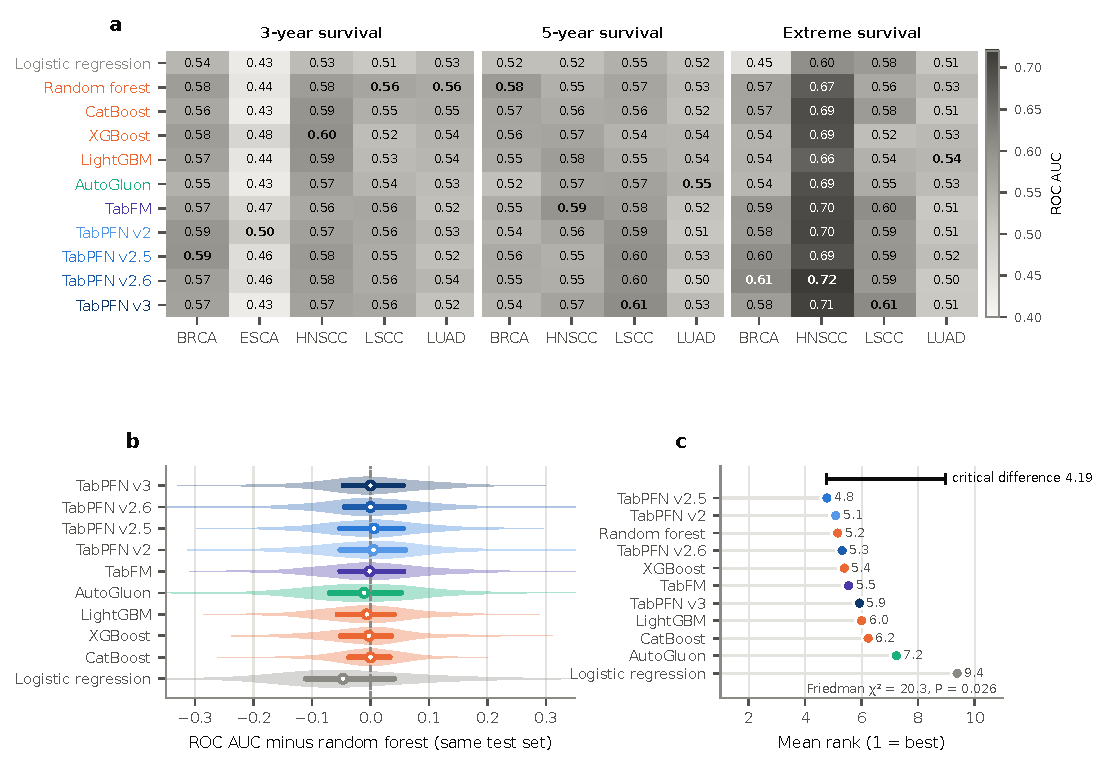
\includegraphics[width=\linewidth,height=0.64\textheight,keepaspectratio]{figures/reusability/fig3_within_cancer.pdf}
\caption{\textbf{Within a single cancer, no model wins decisively.} \textbf{a}, ROC AUC in each of the 13 cancer-specific tasks, grouped by endpoint (3-year, 5-year and extreme survival); each cell is the mean over 25 frozen test sets, and bold marks the best model in each column. \textbf{b}, Paired difference from random forest: distribution of fold-matched ROC AUC differences over the 325 cancer-specific test sets (violin), with interquartile range (bar) and median (circle); the dashed line marks no difference. \textbf{c}, Mean rank of each model across the 13 tasks (1 = best). The bar shows the Nemenyi critical difference at $\alpha = 0.05$; models whose mean ranks differ by less than this are not significantly different. Model names are coloured by family.}
\label{fig:within}
\end{figure}

\subsection*{Pooling lifts every capable model}

Training on all cancers together changed the picture abruptly (Fig.~\ref{fig:pooling}a). For 3-year survival, TabFM reached a mean ROC AUC of 0.721 and TabPFN v3 0.714, while random forest reached 0.716 and CatBoost 0.713. For 5-year survival, TabPFN v3 reached 0.754 against 0.749 for CatBoost, and for extreme survival 0.786 against 0.782. Every nonlinear model gained between 0.14 and 0.22 over its within-cancer level. Logistic regression, restricted to a linear function of the selected features, did not (0.536 at 3 years).

Taken at face value this is the result that motivates pan-cancer modeling. Two features of it argue for caution. The gain was the same size for in-context foundation models, boosted trees and AutoML, more than would be expected from a capacity only some architectures have. And the largest values occurred for extreme survival, which removes the patients with intermediate outcomes and is therefore an easier question rather than a better answer to the fixed-horizon one.

\begin{table}[ht]
\centering
\caption{Mean ROC AUC across frozen test sets. Within-cancer is the average of the three endpoint summaries, each itself averaged over cancers. NA, pooled 3-year training sets exceeded the 1,000-sample CPU limit of TabPFN v2--v2.6.}
\label{tab:model_auc}
\footnotesize\setlength{\tabcolsep}{3pt}\begin{tabular}{llrrrr}
\toprule
Model & Family & Within-cancer & Pooled 3-year & Pooled 5-year & Pooled extreme \\
\midrule
Logistic regression & Linear & 0.524 & 0.536 & 0.542 & 0.522 \\
Random forest & Tree ensemble & 0.561 & 0.716 & 0.747 & 0.781 \\
CatBoost & Boosted tree & 0.559 & 0.713 & 0.749 & 0.782 \\
XGBoost & Boosted tree & 0.556 & 0.701 & 0.734 & 0.768 \\
LightGBM & Boosted tree & 0.554 & 0.698 & 0.719 & 0.762 \\
AutoGluon & AutoML & 0.550 & 0.702 & 0.744 & 0.757 \\
TabFM & Foundation model & 0.565 & 0.721 & 0.753 & 0.780 \\
TabPFN v2 & Foundation model & 0.567 & NA & 0.751 & 0.784 \\
TabPFN v2.5 & Foundation model & 0.568 & NA & 0.753 & 0.785 \\
TabPFN v2.6 & Foundation model & 0.566 & NA & 0.752 & 0.778 \\
TabPFN v3 & Foundation model & 0.563 & 0.714 & 0.754 & 0.786 \\
\bottomrule
\end{tabular}

\end{table}

\subsection*{Controls without patient biology approach the pooled scores}

We then asked how much of the pooled performance remains when patient biology is removed (Fig.~\ref{fig:pooling}b and Table~\ref{tab:shortcuts}). These controls were computed on a single earlier split of the pooled cohorts (141 to 247 test patients), so they place the benchmark scores in context rather than match them. A model given only the patient's cancer type reached ROC AUC 0.707 for 3-year survival, 0.703 for 5-year survival and 0.809 for extreme survival. A model given only the pattern of zero-valued features reached 0.745, 0.704 and 0.824. That pattern mixes measured zeros with features that are structurally absent from a cohort. When survival labels were shuffled within each cancer, preserving each cancer's event rate but removing any link between a patient's profile and outcome, ROC AUC still averaged 0.667, 0.653 and 0.662.

The zero pattern is an almost perfect record of the cohort. From it alone, cancer type was identified with a balanced accuracy of 0.985, against 0.480 from molecular values and 0.20 by chance (Fig.~\ref{fig:pooling}c). In the opposite direction, a linear molecular model trained on four cancers and tested on the fifth reached a mean ROC AUC of 0.479, 0.508 and 0.518 across the three endpoints.

\begin{figure}[tbp]
\centering
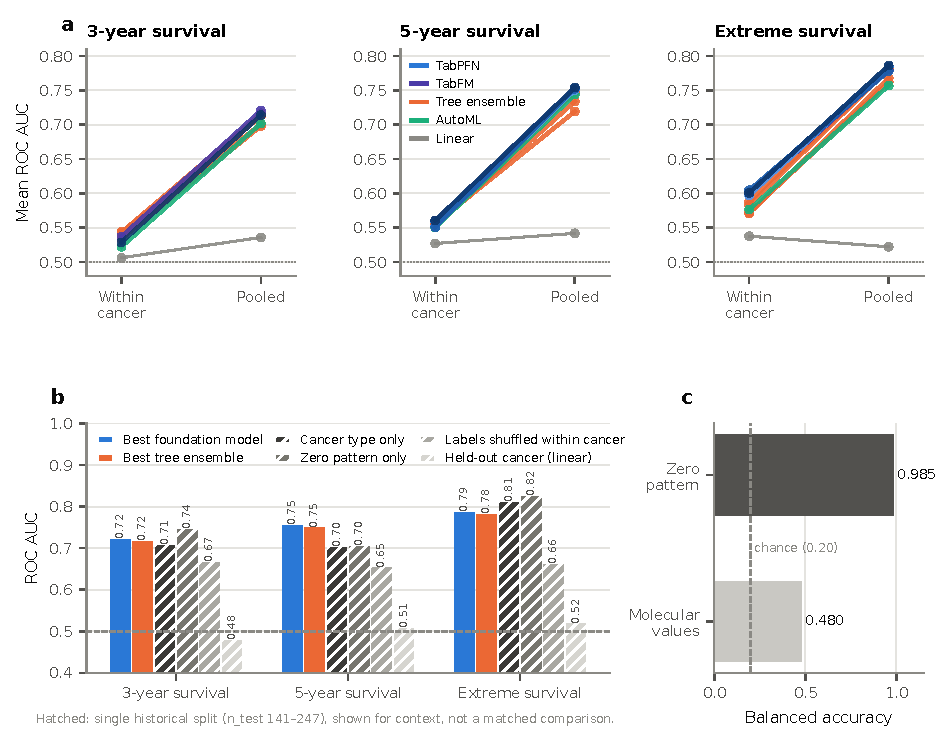
\includegraphics[width=\linewidth,height=0.64\textheight,keepaspectratio]{figures/reusability/fig4_pooling_and_controls.pdf}
\caption{\textbf{Pooling lifts every model, and controls without patient biology reach similar levels.} \textbf{a}, Mean ROC AUC within cancers and in the pooled cohort for each model, by endpoint; lines are coloured by model family. \textbf{b}, Pooled ROC AUC of the best foundation model and the best tree ensemble (solid bars; frozen benchmark) compared with four controls that ignore patient biology: cancer type only, zero pattern only, survival labels shuffled within each cancer (mean of 500 permutations) and a linear model tested on a held-out cancer (mean over held-out cancers). Hatched bars come from a single earlier split and are shown for context, not as a matched comparison. \textbf{c}, How well the cancer type itself can be recovered: balanced accuracy for identifying the cancer from the zero pattern or from molecular values; the dashed line marks chance (0.20 for five cancers).}
\label{fig:pooling}
\end{figure}

\begin{table}[ht]
\centering
\caption{Pooled shortcut and cancer-held-out diagnostics (ROC AUC). Controls were computed on a single earlier split; the best evaluated model is the frozen-benchmark mean for each endpoint. Structural zero denotes the zero-pattern control.}
\label{tab:shortcuts}
\footnotesize\setlength{\tabcolsep}{3pt}\begin{tabular}{lrrrr}
\toprule
Endpoint & Cancer identity & Structural zero & Best evaluated model & Held-out molecular \\
\midrule
3-year OS & 0.707 & 0.745 & 0.721 & 0.479 \\
5-year OS & 0.703 & 0.704 & 0.754 & 0.508 \\
Extreme OS & 0.809 & 0.824 & 0.786 & 0.518 \\
\bottomrule
\end{tabular}

\end{table}

\subsection*{Pooled training lowered within-cancer ranking for foundation models}

A clinician does not rank a breast cancer patient against a lung cancer patient; the diagnosis is already known. The comparison that matters is how well a model ranks patients who share a cancer. Every patient in a pooled task also appears in the corresponding cancer-specific task, so we compared, patient by patient, predictions from a model trained on that cancer alone with predictions from a model trained on the pooled cohort, scoring both only within the cancer.

Pooling did not significantly improve within-cancer ranking for any foundation model, and for several it made ranking worse (Fig.~\ref{fig:effect}a). At 5 years, pooled training lowered the within-cancer ROC AUC of TabFM from 0.540 to 0.456, a change of $-0.084$ (95\% CI, $-0.129$ to $-0.039$), and of TabPFN v3 from 0.539 to 0.469 ($-0.070$; $-0.114$ to $-0.027$). For extreme survival, TabFM fell by 0.081 ($-0.125$ to $-0.032$) and TabPFN v2.6 by 0.068 ($-0.112$ to $-0.023$). Tree ensembles showed smaller estimated changes, at most 0.04 in either direction, with every interval spanning zero. Cancer by cancer, the median change for foundation models was $-0.053$ at 5 years and $-0.036$ for extreme survival, against $-0.010$ and $+0.020$ for tree ensembles; at 3 years both medians were close to zero ($-0.011$ and $-0.020$; Fig.~\ref{fig:effect}b). The only intervals above zero belonged to the two weakest within-cancer models at 3 years, logistic regression ($+0.071$) and AutoGluon ($+0.073$). Of the 30 model--endpoint comparisons, four excluded zero in the negative direction, and all four were foundation models. Because some exclusions are expected by chance across 30 intervals, we place more weight on the direct comparison between families.

Averaged across models, foundation models lost more within-cancer ROC AUC than tree ensembles at every endpoint (Fig.~\ref{fig:effect}c): by 0.027 at 3 years (95\% CI, $-0.060$ to $0.005$), 0.030 at 5 years ($-0.065$ to $0.003$) and 0.042 for extreme survival ($-0.078$ to $-0.005$). Only the extreme-survival difference was resolved by its interval. The consistent direction, together with the four foundation-model exclusions, suggests that pooling degrades within-cancer ranking more for in-context models than for trees. The evidence is consistent but not conclusive.

\begin{figure}[tbp]
\centering
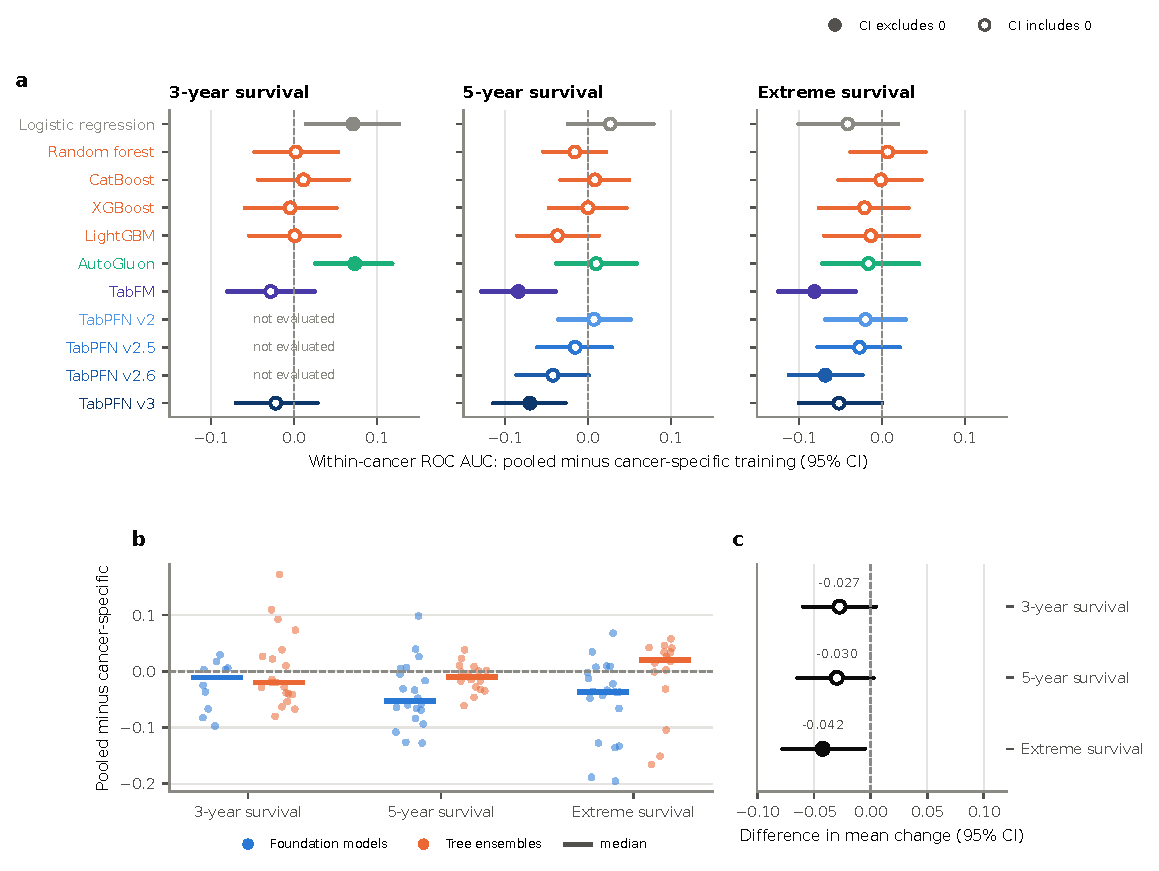
\includegraphics[width=\linewidth,height=0.64\textheight,keepaspectratio]{figures/reusability/fig5_within_cancer_effect.pdf}
\caption{\textbf{Pooled training lowered within-cancer ranking for foundation models.} \textbf{a}, For each model and endpoint, the mean across cancers of the within-cancer ROC AUC of the pooled model minus that of the cancer-specific model, scored on the same patients. Bars are 95\% patient-bootstrap intervals (2,000 resamples, shared across models); filled circles mark intervals that exclude zero. TabPFN v2--v2.6 were not evaluated on pooled 3-year survival. \textbf{b}, The same change shown cancer by cancer: each dot is one model in one cancer, grouped into foundation models and tree ensembles; horizontal bars mark medians. \textbf{c}, Foundation models minus trees: the mean change of foundation models minus that of tree ensembles at each endpoint, with its 95\% interval from the same resamples; a negative value means foundation models lost more.}
\label{fig:effect}
\end{figure}

\FloatBarrier
